\documentclass[a4paper,12pt]{article}
\usepackage[utf8]{inputenc}
\usepackage{graphicx}
\usepackage{enumitem}
\usepackage{hyperref}

\title{Coming-Out-Gruppe für FLINTA\footnote{FLINTA: Frauen, Lesben, Inter-, Nichtbinäre-, Trans-, und Agender Personen} 2024}
\author{}
\date{}

\begin{document}

\maketitle

\section*{Meine persönliche Coming-Out-Geschichte}

Dieses Arbeitsblatt soll dir eine Hilfestellung dabei sein, dich vor allem mit deiner sexuellen/romantischen Orientierung gedanklich zu beschäftigen.  
In den kommenden Sitzungen werden wir uns Zeit nehmen, die persönlichen Geschichten der einzelnen Personen kennen zu lernen.  
Mit Coming-Out–Geschichte ist dabei \textbf{nicht} gemeint, dass du bereits mit anderen über deine Gefühle gesprochen haben musst, die nicht der Erwartung entsprechen, dass Frauen Männer lieben und umgekehrt.  
Hierzu zählen vielmehr auch persönliche Erlebnisse, Erkenntnisse, Begegnungen mit bestimmten Menschen oder mögliche Schlüsselerlebnisse im Laufe des eigenen Lebens, die mit diesen Gefühlen in Zusammenhang stehen.  
Du kannst dazu entweder nur Teil I oder Teil II nutzen oder beide Teile.  
Suche dir einen Ort, an dem du nicht gestört werden kannst, und nimm dir ausreichend Zeit und Ruhe! :)

\section*{Teil 1}

Stelle deine Coming-Out-Geschichte graphisch/bildlich dar. Hier kannst du dich der Mittel bedienen, die dir gerade in den Sinn kommen (z.B. kleine Bildchen, Symbole, kurze Texte, ein Comic, bunte Farben, Muster etc.). Wenn du magst, kannst du auch den unten stehenden Zahlenstrahl (eine oder beide Achsen) nutzen und für dich z.B. als biographische Zeitachse deines Lebens oder was auch immer für dich passend ist beschriften.

\begin{center}
    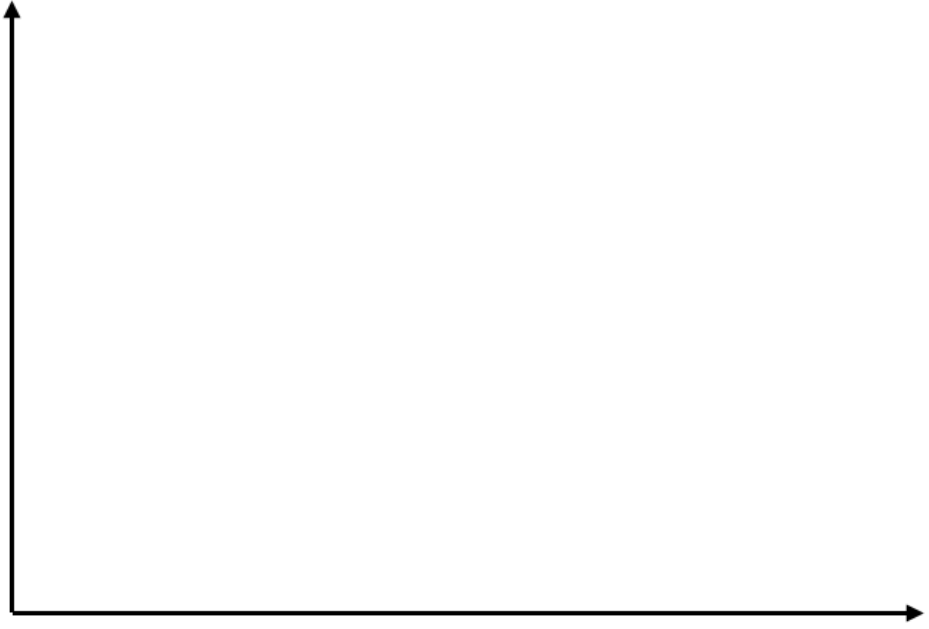
\includegraphics[width=0.8\textwidth]{zeitreihe.png}
\end{center}

\section*{Teil 2}

\begin{quote}
Beantworte alle Fragen, die du gerne beantworten möchtest. Du kannst für einzelne Antworten auch zusätzlich die Rückseite nutzen.
\end{quote}

\begin{enumerate}[label=--]
    \item Wann bzw. Hast du zum ersten Mal Gefühle für eine Person oder mehrere Personen empfunden, die von den gesellschaftlichen Erwartungen an dich abwichen?  

    \rule{12cm}{0.2pt}

    \rule{12cm}{0.2pt}

    \rule{12cm}{0.2pt}
    
    \item Was haben diese Gefühle mit dir gemacht? Wie hast du reagiert?  

    \rule{12cm}{0.2pt}

    \rule{12cm}{0.2pt}
    
    \rule{12cm}{0.2pt}
    
    \item Welche Assoziationen kommen dir bei den Bezeichnungen lesbisch, schwul, bisexuell, pansexuell, asexuell oder aromantisch in den Sinn?  

    \rule{12cm}{0.2pt}

    \rule{12cm}{0.2pt}
    
    \rule{12cm}{0.2pt}
    
    \item Gibt es andere Begriffe, mit denen du dich in letzter Zeit in Bezug auf dich auseinandersetzt?  

    \rule{12cm}{0.2pt}

    \rule{12cm}{0.2pt}
    
    \rule{12cm}{0.2pt}
    
    \item Kennst du Menschen, die offen lesbisch, schwul, bi, pan, asexuell, aromantisch oder in anderer Weise queer\footnote{Queer: Überbegriff für Menschen, die nicht in die romantischen, sexuellen und/oder geschlechtlichen Normen der Gesellschaft passen. Siehe \href{https://queer-lexikon.net/2017/06/08/queer/}{Queer Lexikon}} leben? In welcher Verbindung stehst du zu diesen Personen?  

    \rule{12cm}{0.2pt}

    \rule{12cm}{0.2pt}
    
    \rule{12cm}{0.2pt}
    
    \item Was wünschst du dir bzgl. deiner Gefühle?  

    \rule{12cm}{0.2pt}

    \rule{12cm}{0.2pt}
    
    \rule{12cm}{0.2pt}
\end{enumerate}

\subsection*{Am heutigen Tag ordne ich meine sexuelle und/oder romantische Orientierung auf der Grafik folgendermaßen ein (markiere einen Punkt pro Linie):}

\begin{tabular}{|c|c|c|c|}
    \hline
    \textbf{Zum weiblichen Geschlecht:} & & & \\  
    \hline
    romantisch & gar nicht & \rule{5cm}{0.2pt} & stark \\
    sexuell & gar nicht & \rule{5cm}{0.2pt} & stark \\
    \hline
    \textbf{Zu nichtbinären\footnote{Nichtbinär: Menschen, die sich weder als männlich noch als weiblich identifizieren. Siehe \href{https://queer-lexikon.net/uebersichtsseiten/trans/}{Queer Lexikon}.} Personen:} & & & \\  
    \hline
    romantisch & gar nicht & \rule{5cm}{0.2pt} & stark \\
    sexuell & gar nicht & \rule{5cm}{0.2pt} & stark \\
    \hline
    \textbf{Zum männlichen Geschlecht:} & & & \\  
    \hline
    romantisch & gar nicht & \rule{5cm}{0.2pt} & stark \\
    sexuell & gar nicht & \rule{5cm}{0.2pt} & stark \\
    \hline
\end{tabular}

\begin{enumerate}[label=--]
    \item Gab es bereits Menschen, die deine Gefühle erwidert haben, und oder mit denen du dich zu den oben genannten Themen verbunden und oder verstanden gef\"uhlt hast?  

    \rule{12cm}{0.2pt}
    
    \rule{12cm}{0.2pt}
    
    \rule{12cm}{0.2pt}
    \item Nenne einige Adjektive, die deine Gefühle und Erlebnisse mit Menschen eines Geschlechts beschreiben, zu dem du dich nicht oder vermutlich weniger hingezogen fühlst als erwartet.  
      
    \rule{12cm}{0.2pt}
    
    \rule{12cm}{0.2pt}
    
    \rule{12cm}{0.2pt}
    
    \item Wie ist die Einstellung deiner Eltern gegenüber Menschen, die queer\footnote{Queer: Siehe Fußnote 3.} leben?  

    \rule{12cm}{0.2pt}
    
    \rule{12cm}{0.2pt}

    \rule{12cm}{0.2pt}
    
    \item Hast du das Gefühl, dass die Erwartungen deiner Familie oder deines Umfeldes deine Selbstwahrnehmung beeinflusst haben?  
   
    \rule{12cm}{0.2pt}
    
    \rule{12cm}{0.2pt}
    
    \rule{12cm}{0.2pt}
    
    \item Hast du schon mal mit jemandem über deine Gefühle in Bezug auf deine Identität gesprochen oder sie angedeutet? Wenn ja, wie haben die Personen reagiert?  
    
    \rule{12cm}{0.2pt}
    
    \rule{12cm}{0.2pt}
    
    \rule{12cm}{0.2pt}

    \item Wem würdest du gerne (noch) davon erzählen? Warum? Was erhoffst du dir davon?  

    \rule{12cm}{0.2pt}

    \rule{12cm}{0.2pt}
    
    \rule{12cm}{0.2pt}
    
    \item Welche Medien, Veranstaltungen, Angebote, Filme, Bücher etc. hast du bereits kennengelernt und genutzt, um dich zu informieren? Konntest du dich durch Medien bereits mit deinen Themen auseinandersetzen? Wie hilfreich/weniger hilfreich war das?  
    
    \rule{12cm}{0.2pt}

    \rule{12cm}{0.2pt}
    
    \rule{12cm}{0.2pt}
    
    \item Fühlst du dich gefestigt in deiner Identität, und/oder gibt es Aspekte, die du noch erkunden möchtest?  
    
    \rule{12cm}{0.2pt}
    
    \rule{12cm}{0.2pt}
    
    \rule{12cm}{0.2pt}
    
    \item Was erhoffst du dir für deine persönliche Entwicklung oder deine jetzige Situation allgemein und von deiner Teilnahme an der Gruppe?  
   
    \rule{12cm}{0.2pt}
    
    \rule{12cm}{0.2pt}
    
    \rule{12cm}{0.2pt}
    
    \item \textbf{Worauf freust du dich?}  
   
    \rule{12cm}{0.2pt}

    \rule{12cm}{0.2pt}
    
    \rule{12cm}{0.2pt}
\end{enumerate}

\end{document}
